\documentclass[a4paper]{article}
\usepackage[T1]{fontenc}			% \chapter package
\usepackage[english]{babel}
\usepackage[english]{isodate}  		% date format
\usepackage{graphicx}				% manage images
\usepackage{amsfonts}
\usepackage{booktabs}				% high quality tables
\usepackage{amsmath}				% math package
\usepackage{amssymb}				% another math package (e.g. \nexists)
\usepackage{bm}                     % bold math symbols
\usepackage{mathtools}				% emphasize equations
\usepackage{stmaryrd} 				% '\llbracket' and '\rrbracket'
\usepackage{amsthm}					% better theorems
\usepackage{enumitem}				% manage list
\usepackage{pifont}					% nice itemize
\usepackage{cancel}					% cancel math equations
\usepackage{caption}				% custom caption
\usepackage[]{mdframed}				% box text
\usepackage{multirow}				% more lines in a table
\usepackage{textcomp, gensymb}		% degree symbol
\usepackage[x11names]{xcolor}		% RGB color
\usepackage[many]{tcolorbox}		% colorful box
\usepackage{multicol}				% more rows in a table (used for the lists)
\usepackage{listings}
\usepackage{url}
\usepackage{qrcode}
\usepackage{fontawesome5}
\usepackage{ragged2e}
\usepackage{cite}                   % references
\usepackage{imakeidx}               % index
\makeindex[program=makeindex, columns=1,
           title=Index, 
           intoc,
           options={-s index-style.ist}]
\usepackage{fancyhdr}

%\pdfcompresslevel=0
%\pdfobjcompresslevel=0

\definecolor{codegreen}{rgb}{0,0.6,0}
\definecolor{codegray}{rgb}{0.5,0.5,0.5}
\definecolor{codepurple}{rgb}{0.58,0,0.82}
\definecolor{backcolour}{rgb}{0.95,0.95,0.92}
\lstdefinestyle{mystyle}{
    backgroundcolor=\color{backcolour},
    commentstyle=\color{codegreen},
    keywordstyle=\color{magenta},
    numberstyle=\tiny\color{codegray},
    stringstyle=\color{codepurple},
    basicstyle=\ttfamily\footnotesize,
    breakatwhitespace=false,
    breaklines=true,
    captionpos=b,
    keepspaces=true,
    numbers=left,
    numbersep=5pt,
    showspaces=false,
    showstringspaces=false,
    showtabs=false,
    tabsize=2
}
\lstset{style=mystyle}


% thanks Mico: https://tex.stackexchange.com/a/60218/312896
\makeatletter
\renewcommand\paragraph{\@startsection{paragraph}{4}{\z@}%
            {-2.5ex\@plus -1ex \@minus -.25ex}%
            {1.25ex \@plus .25ex}%
            {\normalfont\normalsize\bfseries}}
\makeatother
\setcounter{secnumdepth}{4} % how many sectioning levels to assign numbers to
\setcounter{tocdepth}{4}    % how many sectioning levels to show in ToC


% draw a frame around given text
\newcommand{\framedtext}[1]{%
	\par%
	\noindent\fbox{%
		\parbox{\dimexpr\linewidth-2\fboxsep-2\fboxrule}{#1}%
	}%
}


% table of content links
\usepackage{xcolor}
\usepackage[linkcolor=black, citecolor=blue, urlcolor=cyan]{hyperref} % hypertexnames=false
\hypersetup{
	colorlinks=true
}


\newtheorem{theorem}{\textcolor{Red3}{\underline{Theorem}}}
\renewcommand{\qedsymbol}{QED}
\newcommand{\dquotes}[1]{``#1''}
\newcommand{\longline}{\noindent\rule{\textwidth}{0.4pt}}
\newcommand{\circledtext}[1]{\raisebox{.5pt}{\textcircled{\raisebox{-.9pt}{#1}}}}
\newcommand{\definition}[1]{\textcolor{Red3}{\textbf{#1}}\index{#1}}
\newcommand{\definitionWithSpecificIndex}[2]{\textcolor{Red3}{\textbf{#1}}\index{#2}}
\newcommand{\example}[1]{\textcolor{Green4}{\textbf{#1}}}
\newcommand{\highspace}{\vspace{1.2em}\noindent}
\newcommand{\version}{v0.1.0}
\newcommand{\nnz}{\mathrm{nnz}} % non-zero entries


\begin{document}
    \newcounter{definition}[section]
    \newcounter{example}[section]
    \newcounter{exercise}[section]
    
    \newtcolorbox[use counter = definition]{definitionbox}[1][]{%
        breakable,
        enhanced,
        colback=red!5!white,
        colframe=red!75!black,
        fonttitle=\bfseries,
        title={Definition \thetcbcounter#1} %
    }

    \newtcolorbox[use counter = exercise]{exercisebox}[1][]{%
        breakable,
        enhanced,
        colback=Red3!5!white,
        colframe=Red3!75!black,
        fonttitle=\bfseries,
        title={Exercise \thetcbcounter#1} %
    }
    
    \newtcolorbox[use counter = example]{examplebox}[1][]{%
        breakable,
        enhanced,
        colback=Green4!5!white,
        colframe=Green4!75!black,
        fonttitle=\bfseries,
        title={Example \thetcbcounter#1} %
    }

    \newtcolorbox[]{deepeningbox}[1][]{%
        breakable,
        enhanced,
        colback=DarkOrange3!5!white,
        colframe=DarkOrange3!75!black,
        fonttitle=\bfseries,
        title={Deepening#1} %
    }

    %%%%%%%%%%%%%%%
    % Notes cover %
    %%%%%%%%%%%%%%%
    \author{260236}
\title{Parallel Computing - Notes - \version}
\date{\printdayoff\today}
\maketitle

    %%%%%%%%%%%
    % Preface %
    %%%%%%%%%%%
	\section*{Preface}

Every theory section in these notes has been taken from the sources:
\begin{itemize}
    \item Course slides.\cite{numerical-linear-algebra-polimi}
\end{itemize}
About:
\begin{itemize}
    \item[\faIcon{github}] \href{https://github.com/PoliMI-HPC-E-notes-projects-AndreVale69/HPC-E-PoliMI-university-notes}{GitHub repository}
    \begin{center}
        \qrcode{https://github.com/PoliMI-HPC-E-notes-projects-AndreVale69/HPC-E-PoliMI-university-notes}
    \end{center}
\end{itemize}
These notes are an unofficial resource and shouldn't replace the course material or any other book on numerical linear algebra. It is not made for commercial purposes. I've made the following notes to help me improve my knowledge and maybe it can be helpful for everyone.

As I have highlighted, a student should choose the teacher's material or a book on the topic. These notes can only be a helpful material.

\highspace

\subsection*{Correlated Projects}

During the Numerical Linear Algebra for HPC course, I was part of a team where we created a project that included two challenges related to the course. See more details in the corresponding repository:
\begin{itemize}
    \item[\faIcon{github}] \href{https://github.com/PoliMI-HPC-E-notes-projects-AndreVale69/NLA-challenges}{GitHub repository}
    \begin{center}
        \qrcode{https://github.com/PoliMI-HPC-E-notes-projects-AndreVale69/NLA-challenges}
    \end{center}
\end{itemize}

    %%%%%%%%%%%%%%%%%%%%%
    % Table of contents %
    %%%%%%%%%%%%%%%%%%%%%
    \tableofcontents
    \newpage

    %%%%%%%%%%%%%%%%%%%
    % Fancy pagestyle %
    %%%%%%%%%%%%%%%%%%%
    \pagestyle{fancy}
    \fancyhead{} % clear all header fields
    \fancyhead[R]{\nouppercase{\leftmark\hfill\rightmark}}
    
    %%%%%%%%%%%%%%%%%
    % Preliminaries %
    %%%%%%%%%%%%%%%%%
    \section{Preliminaries}

This section introduces some of the basic topics used throughout the course.

\subsection{Notation}

    \subsection{Matrix Operations}

Some basic matrix operations:
\begin{itemize}
	\item \textbf{Inner products}. If $\mathbf{x}, \mathbf{y} \in \mathbb{R}^{n}$ then:
	\begin{equation*}
		\mathbf{x}^{T} \mathbf{y} = \displaystyle\sum_{i = 1, \dots, n} x_{i}y_{i}
	\end{equation*}
	For real vectors, the commutative property is true:
	\begin{equation*}
		\mathbf{x}^{T} \mathbf{y} = \mathbf{y}^{T} \mathbf{x}
	\end{equation*}
	Furthermore, the vectors $\mathbf{x}, \mathbf{y} \in \mathbb{R}^{n}$ are \textbf{orthogonal} if:\index{Orthogonal Vectors}
	\begin{equation*}
		\mathbf{x}^{T} \mathbf{y} = \mathbf{y}^{T} \mathbf{x} = \mathbf{0}
	\end{equation*}
	And finally, some useful properties of matrix multiplication:
	\begin{enumerate}
		\item Multiplication by the \emph{identity} changes nothing.
		\begin{equation*}\index{Matrices Multiplication}
			A \in \mathbb{R}^{n \times m} \: \Rightarrow \: \mathbf{I}_{n} A = A = A\mathbf{I}_{m}
		\end{equation*}
		
		\item Associativity:
		\begin{equation*}\index{Matrix Associativity Property}
			A\left(BC\right) = \left(AB\right)C
		\end{equation*}
		
		\item Distributive:
		\begin{equation*}\index{Matrix Distributive Property}
			A\left(B+D\right) = AB + AD
		\end{equation*}
		
		\item \underline{No} commutativity:
		\begin{equation*}
			AB \ne BA
		\end{equation*}
		
		\item Transpose of product:
		\begin{equation*}\index{Transpose product between matrices}
			\left(AB\right)^{T} = B^{T} A^{T}
		\end{equation*}
	\end{enumerate}
	
	\item \textbf{Matrix powers}. For $A \in \mathbb{R}^{n \times n}$ with $A \ne \mathbf{0}$:
	\begin{equation*}
		A^{0} = \mathbf{I}_{n} \hspace{2em} A^{k} = \underbrace{A \cdots A}_{k\text{ times}} = AA^{k-1} \hspace{2em} k \ge 1
	\end{equation*}
	Furthermore, $A \in \mathbb{R}^{n \times n}$ is:
	\begin{itemize}
		\item \textbf{Idempotent} (projector) $A^{2} = A$ \index{Idempotent Matrices}
		\item \textbf{Nilpotent} $A^{k} = \mathbf{0}$ for some integer $k \ge 1$ \index{Nilpotent Matrices}
	\end{itemize}
	
	\item \textbf{Inverse}. For $A \in \mathbb{R}^{n \times n}$ is \definitionWithSpecificIndex{non-singular}{Non-singular Matrices} (\definitionWithSpecificIndex{invertible}{Invertible Matrices}), if exists $A^{-1}$ with:
	\begin{equation}\label{eq: non-singular matrix}
		AA^{-1} = \mathbf{I}_{n} = A^{-1}A
	\end{equation}
	Inverse and transposition are interchangeable:
	\begin{equation*}
		A^{-T} \triangleq \left(A^{T}\right)^{-1} = \left(A^{-1}\right)^{T}
	\end{equation*}
	Furthermore, an inverse of a product for a matrix $A \in \mathbb{R}^{n \times n}$ can be expressed as:
	\begin{equation*}
		\left(AB\right)^{-1} = B^{-1}A^{-1}
	\end{equation*}
	Finally, remark that if $\mathbf{0} \ne \mathbf{x} \in \mathbb{R}^{n}$ and $A\mathbf{x} = 0$, then $A$ is \definitionWithSpecificIndex{singular}{Singular Matrices}.
	
	\item \textbf{Orthogonal matrices}. Given a matrix $A \in \mathbb{R}^{n \times n}$ that is \emph{invertible}, the matrix $A$ is said to be \definitionWithSpecificIndex{orthogonal}{Orthogonal Matrices} if:
	\begin{equation*}
		A^{-1} = A^{T} \: \Rightarrow \: A^{T}A = \mathbf{I}_{n} = AA^{T}
	\end{equation*}
	
	\item \textbf{Triangular matrices}. There are two types of triangular matrices:
	\begin{enumerate}
		\item \definition{Upper triangular matrix}:
		\begin{equation*}
			\mathbf{U} = \begin{bmatrix}
				u_{1,1} & u_{1,2} & \cdots & u_{1,n} \\
				0 & u_{2,2} & \cdots & u_{2,n} \\
				\vdots & \cdots & \ddots & \vdots \\
				0 & 0 & \cdots & u_{n,n} \\
			\end{bmatrix}
		\end{equation*}
		$\mathbf{U}$ is \textbf{non-singular} if and only if $u_{ii} \ne 0$ for $i = 1, \dots, n$.

		\item \definition{Lower triangular matrix}:
		\begin{equation*}
			\mathbf{L} = \begin{bmatrix}
				l_{1,1} & 0 & \cdots & 0 \\
				l_{2,1} & l_{2,2} & \cdots & 0 \\
				\vdots & \cdots & \ddots & \vdots \\
				l_{n,1} & l_{n,2} & \cdots & l_{n,n} \\
			\end{bmatrix}
		\end{equation*}
		$\mathbf{L}$ is \textbf{non-singular} if and only if $l_{ii} \ne 0$ for $i = 1, \dots, n$.
	\end{enumerate}
	
	\item \textbf{Unitary triangular matrices}. Are matrices similar to the lower and upper matrices, but they have the main diagonal composed of ones.
	\begin{enumerate}
		\item \definition{Unitary upper triangular matrix}:
		\begin{equation*}
			\mathbf{U} = \begin{bmatrix}
				1 & u_{1,2} & \cdots & u_{1,n} \\
				0 & 1 & \cdots & u_{2,n} \\
				\vdots & \cdots & \ddots & \vdots \\
				0 & 0 & \cdots & 1 \\
			\end{bmatrix}
		\end{equation*}

		\item \definition{Unitary lower triangular matrix}:
		\begin{equation*}
			\mathbf{L} = \begin{bmatrix}
				1 & 0 & \cdots & 0 \\
				l_{2,1} & 1 & \cdots & 0 \\
				\vdots & \cdots & \ddots & \vdots \\
				l_{n,1} & l_{n,2} & \cdots & 1 \\
			\end{bmatrix}
		\end{equation*}
	\end{enumerate}
\end{itemize}
    \subsection{Basic matrix decomposition}

In the Numerical Linear Algebra course, we will use three main decomposition:
\begin{itemize}
	\item \underline{\textbf{LU factorization with (partial) pivoting}}. If $A \in \mathbb{R}^{n \times n}$ is a non-singular matrix, then:
	\begin{equation*}
		PA = LU
	\end{equation*}
	Where:
	\begin{itemize}
		\item $P$ is a permutation matrix
		\item $L$ is an unit lower triangular matrix
		\item $U$ is an upper triangular matrix
	\end{itemize}
	Note that the linear system solution:
	\begin{equation*}
		A\mathbf{x} = \mathbf{b}
	\end{equation*}
	Can be solved directly by calculation:
	\begin{equation*}
		PA = LU
	\end{equation*}
	This way the complexity is equal to $O\left(n^{3}\right)$. So a smarter way to reduce complexity is to use the \emph{divide et impera} (or \emph{divide and conquer}) technique. Then solve the system:
	\begin{equation*}
		\begin{cases}
			L\mathbf{y} = P\mathbf{b} & \rightarrow \text{ unit lower triangular system, complexity } O\left(n^{2}\right) \\
			U\mathbf{x} = \mathbf{y}  & \rightarrow \text{ upper triangular system, complexity } O\left(n^{2}\right)
		\end{cases}
	\end{equation*}

	\item \underline{\textbf{Cholesky decomposition}}. If $A \in \mathbb{R}^{n \times n}$ is a symmetric\footnote{$A^{T} = A$} and positive definite\footnote{$\mathbf{z}^{T} A \mathbf{z} > 0 \hspace{2em} \forall \mathbf{z} \ne 0$}, then:
	\begin{equation*}
		A = L^{T}L
	\end{equation*}
	Where $L$ is a lower triangular matrix (with positive entries on the diagonal). Also note that the linear system solution:
	\begin{equation*}
		A\mathbf{x} = \mathbf{b}
	\end{equation*}
	Can be solved directly by calculation:
	\begin{equation*}
		A = L^{T}L
	\end{equation*}
	This way the complexity is equal to $O\left(n^{3}\right)$. So a smarter way to reduce complexity is to use the \emph{divide et impera} (or \emph{divide and conquer}) technique. Then solve the system:
	\begin{equation*}
		\begin{cases}
			L^{T}\mathbf{y} = \mathbf{b} & \rightarrow \text{ lower triangular system, complexity } O\left(n^{2}\right) \\
			L\mathbf{x} = \mathbf{y}  & \rightarrow \text{ upper triangular system, complexity } O\left(n^{2}\right)
		\end{cases}
	\end{equation*}

	\item \underline{\textbf{QR decomposition}}. If $A \in \mathbb{R}^{n \times n}$ is a non-singular matrix, then:
	\begin{equation*}
		A = QR
	\end{equation*}
	Where:
	\begin{itemize}
		\item $Q$ is an orthogonal matrix
		\item $R$ is an upper triangular
	\end{itemize}
	Note that the linear system solution:
	\begin{equation*}
		A\mathbf{x} = \mathbf{b}
	\end{equation*}
	Can be solved directly by calculation:
	\begin{equation*}
		A = QR
	\end{equation*}
	This way the complexity is equal to $O\left(n^{3}\right)$. So a smarter way to reduce complexity is to use the \emph{divide et impera} (or \emph{divide and conquer}) technique. Then:
	\begin{enumerate}
		\item Multiply $\mathbf{c} = Q^{T}\mathbf{b}$, complexity $O\left(n^{2}\right)$
		
		\item Solve the lower triangular system $R\mathbf{x} = \mathbf{c}$, complexity $O\left(n^{2}\right)$
	\end{enumerate}
\end{itemize}
    \subsection{Determinants}

We will assume that the determinant topic is well known. However, in the following enumerated list there are some useful properties about the determinant of a matrix:
\begin{enumerate}
	\item If a general matrix $T \in \mathbb{R}^{n \times n}$ is upper- or lower-triangular, then the determinant is computed as:
	\begin{equation*}
		\det\left(T\right) = \displaystyle\prod_{i = 1}^{n} t_{i,i}
	\end{equation*}
	
	\item Let $A,B \in \mathbb{R}^{n \times n}$, then is true:
	\begin{equation*}
		\det\left(AB\right) = \det\left(A\right) \cdot \det\left(B\right)
	\end{equation*}
	
	\item Let $A \in \mathbb{R}^{n \times n}$, then is true:
	\begin{equation*}
		\det\left(A^{T}\right) = \det\left(A\right)
	\end{equation*}
	
	\item Let $A \in \mathbb{R}^{n \times n}$, then is true:
	\begin{equation*}
		\det\left(A\right) \ne 0 \iff A \text{ is non-singular}
	\end{equation*}
	
	\item \textbf{Computation}. Let $A \in \mathbb{R}^{n \times n}$ be non-singular, then:
	\begin{enumerate}
		\item Factor $PA = LU$
		\item $\det\left(A\right) = \pm\det\left(U\right) = \pm u_{1,1} \dots u_{n,n}$
	\end{enumerate}
\end{enumerate}
    \subsection{Sparse matrices}

A \definitionWithSpecificIndex{sparse matrix}{Sparse Matrix} is a matrix in which most of the elements are zero; roughly speaking, given $A \in \mathbb{R}^{n \times n}$, the number of non-zero entries of $A$ (denoted $\nnz\left(A\right)$) is $O\left(n\right)$, we say that $A$ is \textbf{sparse}.

\highspace
Sparse matrices are so important because when we try to solve:
\begin{equation*}
	A \mathbf{x} = \mathbf{b}
\end{equation*}
The $A$ matrix is often sparse, especially when it comes from the discretization of partial differential equations.

\highspace
Finally, note that the iterative methods (explained in the next section) only use a sparse matrix $A$ in the context of the matrix-vector product. Then we only need to provide the matrix-vector product to the computer.

\longline

\subsubsection{Storage schemes}

Unfortunately, storing a sparse matrix is a waste of memory. Instead of storing a dense array (with many zeros), the main idea is to \textbf{store only the non-zero entries, plus their locations}.

\highspace
This technique allows to save data storage because it will be from $O\left(n^{2}\right)$ to $O\left(\nnz\right)$.

\highspace
The most common sparse storage types are:
\begin{itemize}
	\item \definition{Coordinate format (COO)}. The data structure consists of three arrays (of length $\nnz\left(A\right)$):
	\begin{itemize}
		\item \texttt{AA}: all the values of the non-zero elements of $A$ in any order.
		
		\item \texttt{JR}: integer array containing their row indices.
		
		\item \texttt{JC}: integer array containing their column indices.
	\end{itemize}
	For \example{example}:
	\begin{equation*}
		A = \begin{bmatrix}
			1. & 0. & 0.& 2. & 0. \\
			3. & 4. & 0.& 5. & 0. \\
			6. & 0. & 7.& 8. & 9. \\
			0. & 0. & 10.& 11. & 0. \\
			0. & 0. & 0.& 0. & 12. 
		\end{bmatrix}
	\end{equation*}
	\begin{equation*}
		\begin{array}{rcl}
			\texttt{AA} &=& \left[
				12.\hspace{1em}
				9.\hspace{1em}
				7.\hspace{1em}
				5.\hspace{1em}
				1.\hspace{1em}
				2.\hspace{1em}
				11.\hspace{1em}
				3.\hspace{1em}
				6.\hspace{1em}
				4.\hspace{1em}
				8.\hspace{1em}
				10.
			\right] \\ [.5em]
			\texttt{JR} &=& \left[
				\phantom{1}5\phantom{.}\hspace{1em}
				3\phantom{.}\hspace{1em}
				3\phantom{.}\hspace{1em}
				2\phantom{.}\hspace{1em}
				1\phantom{.}\hspace{1em}
				1\phantom{.}\hspace{1em}
				\phantom{1}4\phantom{.}\hspace{1em}
				2\phantom{.}\hspace{1em}
				3\phantom{.}\hspace{1em}
				2\phantom{.}\hspace{1em}
				3\phantom{.}\hspace{1em}
				\phantom{1}4\phantom{.}
			\right] \\ [.5em]
			\texttt{JC} &=& \left[
				\phantom{1}5\phantom{.}\hspace{1em}
				5\phantom{.}\hspace{1em}
				3\phantom{.}\hspace{1em}
				4\phantom{.}\hspace{1em}
				1\phantom{.}\hspace{1em}
				4\phantom{.}\hspace{1em}
				\phantom{1}4\phantom{.}\hspace{1em}
				1\phantom{.}\hspace{1em}
				1\phantom{.}\hspace{1em}
				2\phantom{.}\hspace{1em}
				4\phantom{.}\hspace{1em}
				\phantom{1}3\phantom{.}
			\right]
		\end{array}
	\end{equation*}
	\newpage
	\begin{figure}[!htp]
		\centering
		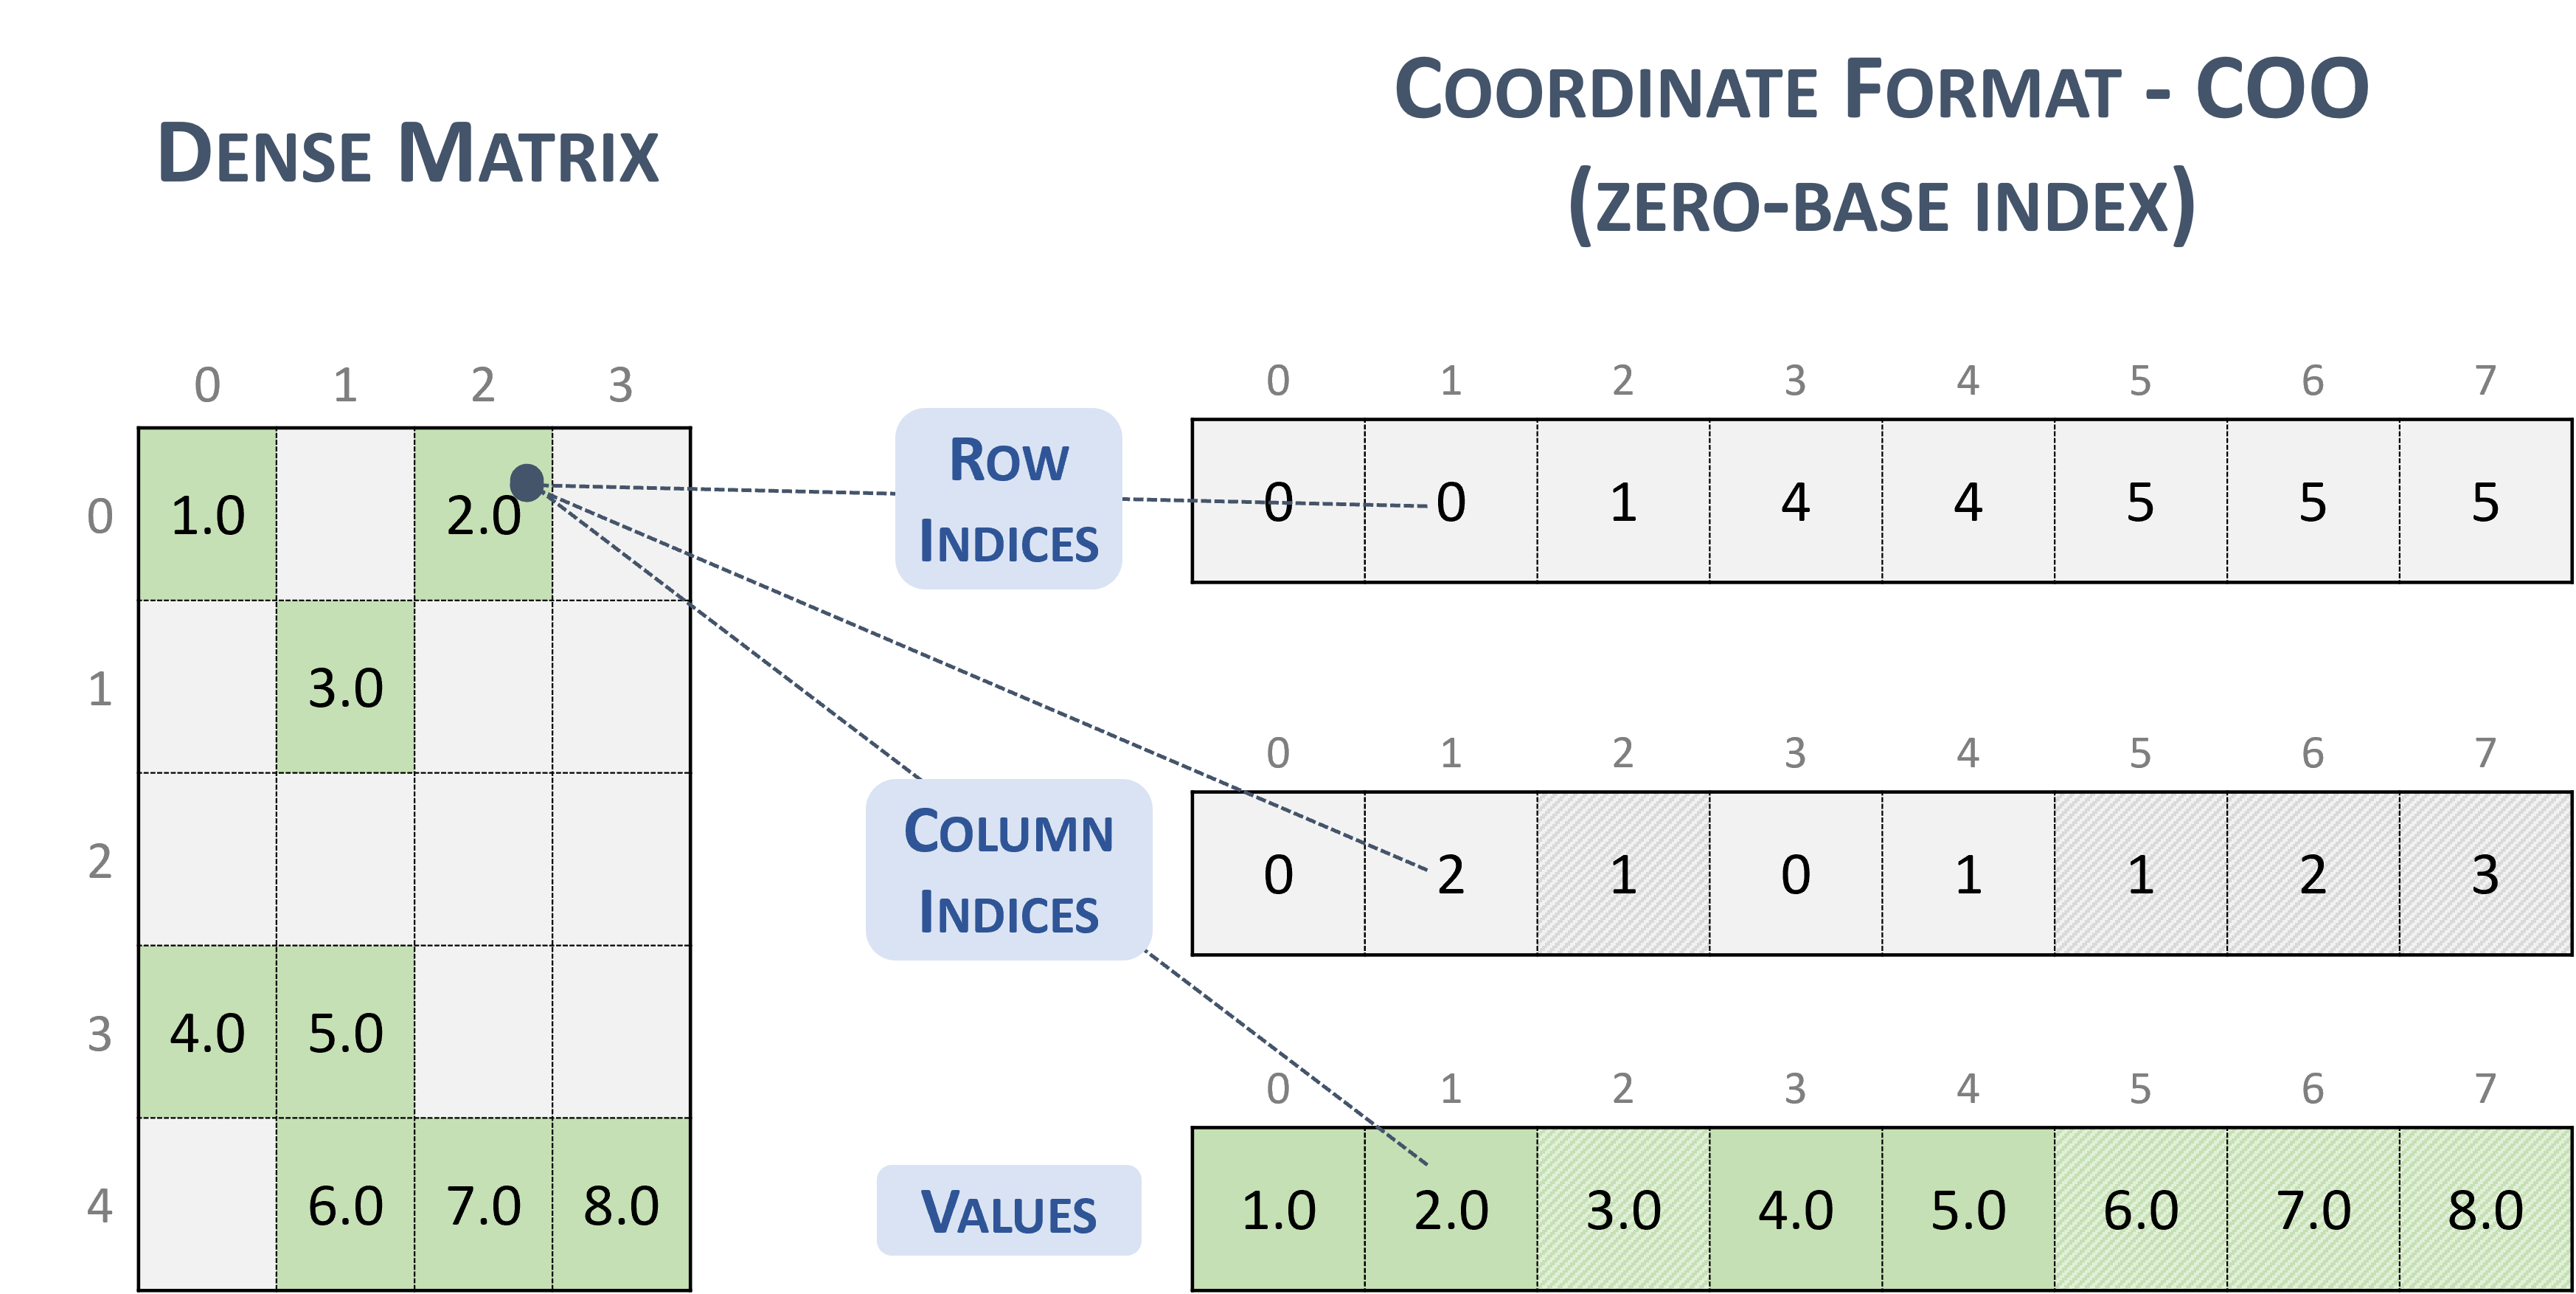
\includegraphics[width=\textwidth]{img/coo.png}
		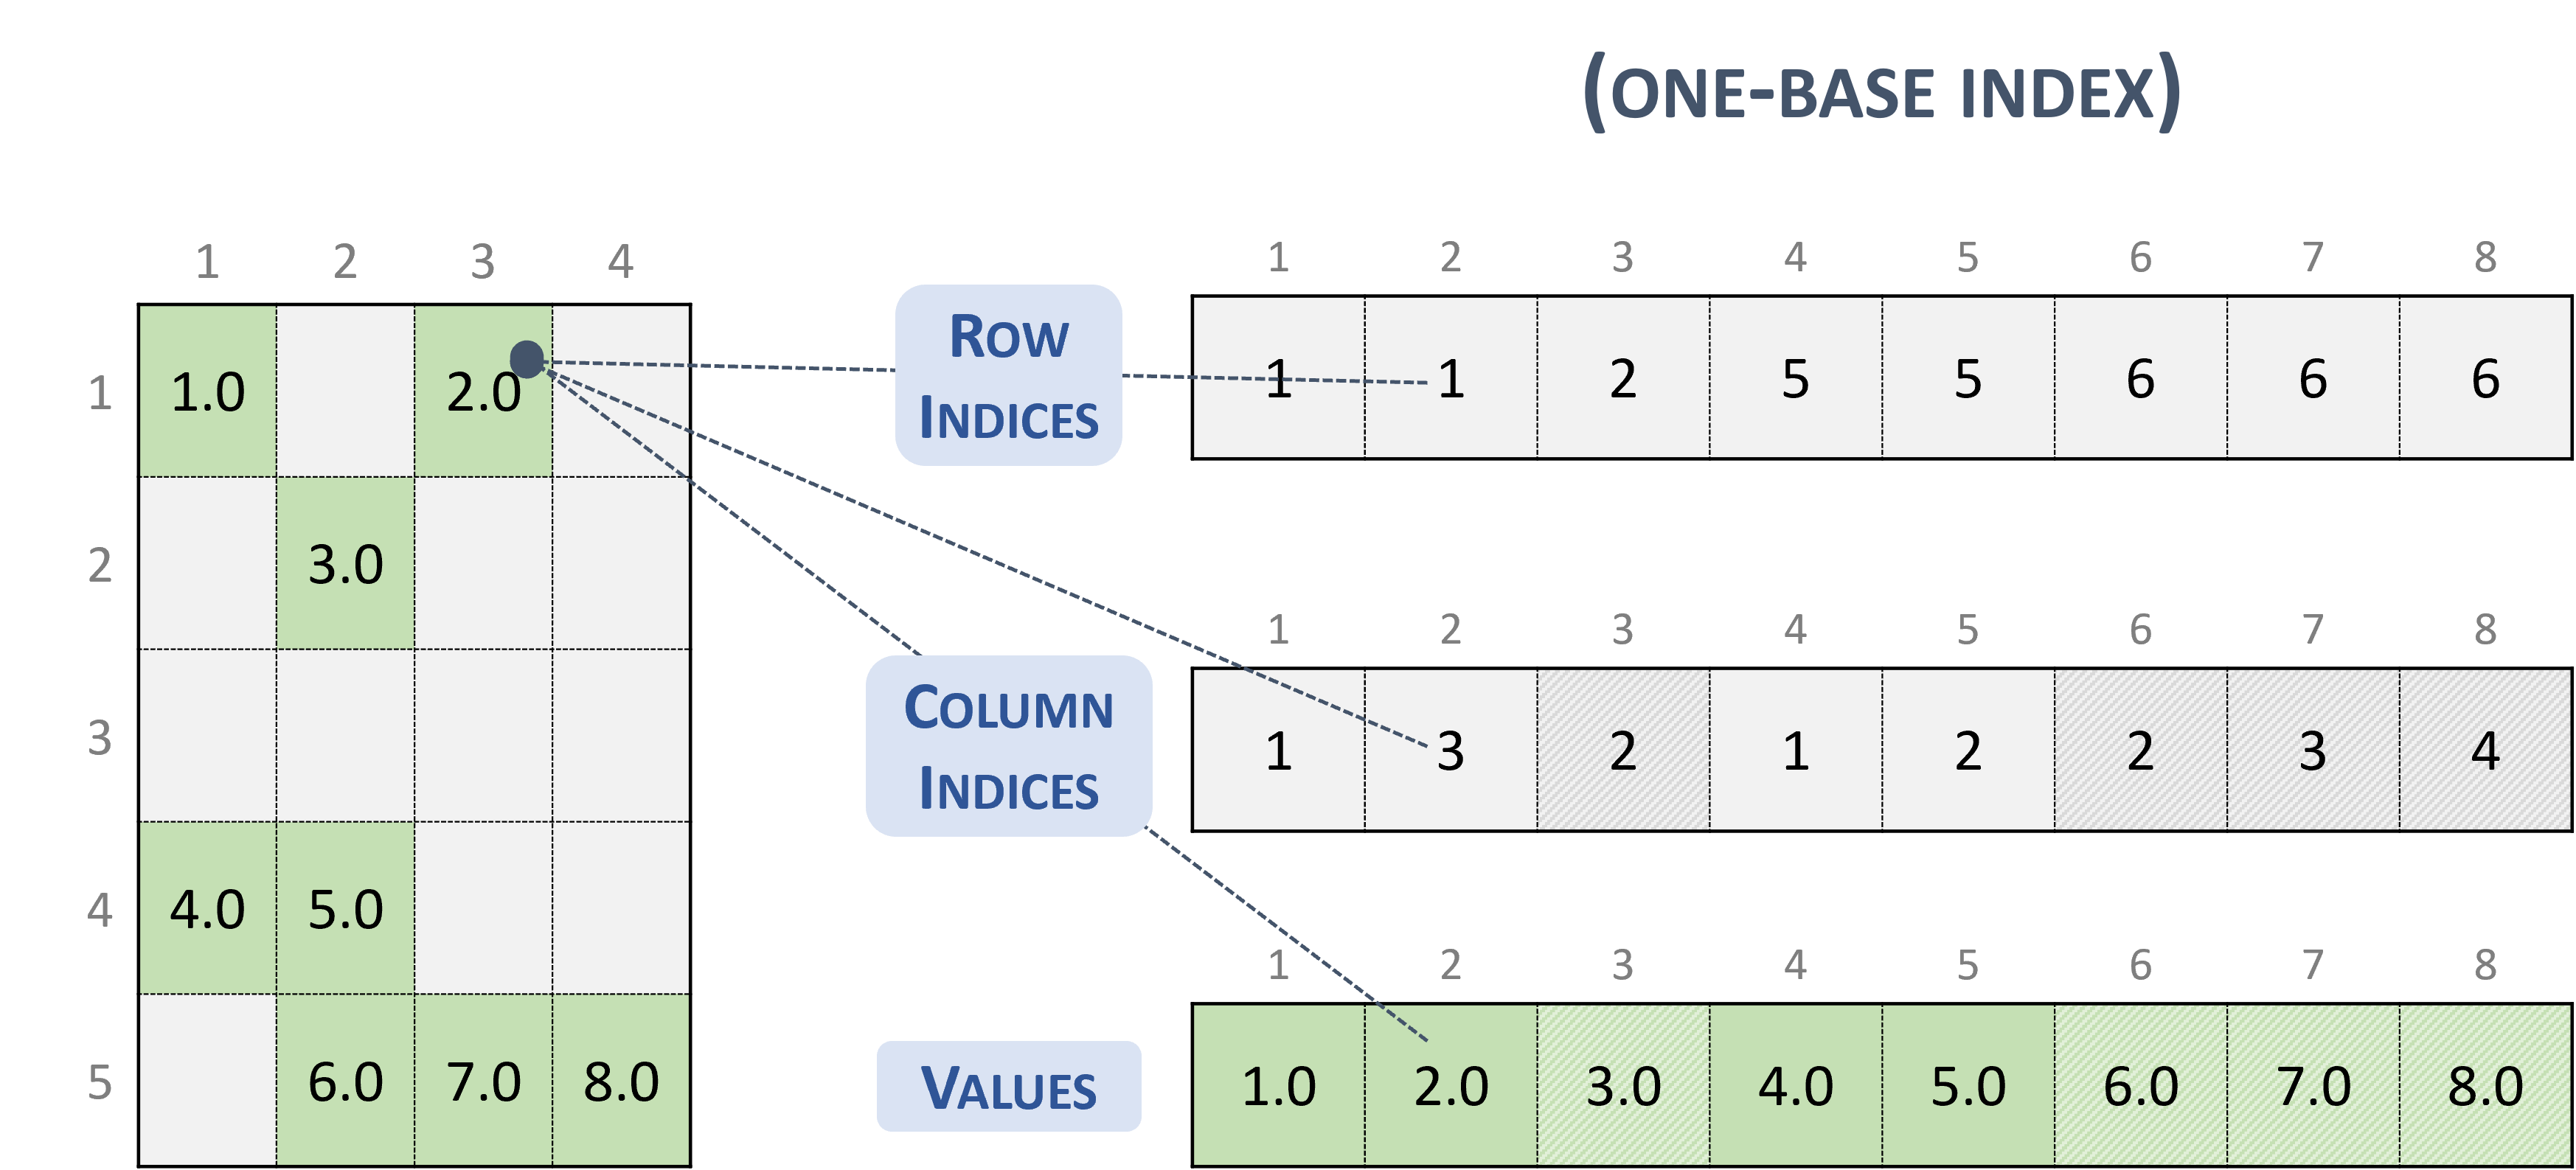
\includegraphics[width=\textwidth]{img/coo_one_base.png}
		\caption{Graphical representation of the coordinate format (COO) technique. From the figure we can see the representation of the \texttt{AA} array, called \emph{values}, the \texttt{JR}, called \emph{row indices}, and finally the \texttt{JC}, called \emph{column indices}. The algorithm is very simple. The figures are taken from the \href{https://docs.nvidia.com/nvpl/_static/sparse/storage_format/sparse_matrix.html}{NVIDIA Performance Libraries Sparse}, which is part of the \href{https://developer.nvidia.com/nvpl}{NVIDIA Performance Libraries}.}
	\end{figure}
	
	\item \definition{Coordinate Compressed Sparse Row format (CSR)}. If the elements of $A$ are listed by row, the array \texttt{JC} might be replaced by an array that points to the beginning of each row.
	\begin{itemize}
		\item \texttt{AA}: all the values of the non-zero elements of $A$, stored row by row from $1, \dots, n$.
		
		\item \texttt{JA}: contains the column indices.
		
		\item \texttt{IA}: contains the pointers to the beginning of each row in the arrays $A$ and \texttt{JA}. Thus \texttt{IA}$\left(i\right)$ contains the position in the arrays \texttt{AA} and \texttt{JA} where the $i$-th row starts. The length of \texttt{IA} is $n+1$, with $\texttt{IA}\left(n+1\right)$ containing the number $A\left(1\right) + \nnz\left(A\right)$. Remember that $n$ is the number of rows.
	\end{itemize}
	For \example{example}:
	\begin{equation*}
		A = \begin{bmatrix}
			1. & 0. & 0.& 2. & 0. \\
			3. & 4. & 0.& 5. & 0. \\
			6. & 0. & 7.& 8. & 9. \\
			0. & 0. & 10.& 11. & 0. \\
			0. & 0. & 0.& 0. & 12. 
		\end{bmatrix}
	\end{equation*}
	\begin{equation*}
		\begin{array}{rcl}
			\texttt{AA} &=& \left[
				1.\hspace{1em}
				2.\hspace{1em}
				3.\hspace{1em}
				\phantom{1}4.\hspace{1em}
				\phantom{1}5.\hspace{1em}
				\phantom{1}6.\hspace{1em}
				7.\hspace{1em}
				8.\hspace{1em}
				9.\hspace{1em}
				10.\hspace{1em}
				11.\hspace{1em}
				12.
			\right] \\ [.5em]
			\texttt{JA} &=& \left[
				1\phantom{.}\hspace{1em}
				4\phantom{.}\hspace{1em}
				1\phantom{.}\hspace{1em}
				\phantom{1}2\phantom{.}\hspace{1em}
				\phantom{1}4\phantom{.}\hspace{1em}
				\phantom{1}1\phantom{.}\hspace{1em}
				3\phantom{.}\hspace{1em}
				4\phantom{.}\hspace{1em}
				5\phantom{.}\hspace{1em}
				\phantom{1}3\phantom{.}\hspace{1em}
				\phantom{1}4\phantom{.}\hspace{1em}
				\phantom{1}5\phantom{.}
			\right] \\ [.5em]
			\texttt{IA} &=& \left[
				1\phantom{.}\hspace{1em}
				3\phantom{.}\hspace{1em}
				6\phantom{.}\hspace{1em}
				10\phantom{.}\hspace{1em}
				12\phantom{.}\hspace{1em}
				13\phantom{.}
			\right]
		\end{array}
	\end{equation*}
	To retrieve each position of the matrix, the algorithm is quite simple. Consider the \texttt{IA} arrays. 
	\begin{enumerate}
		\item We start at position one of the array, then the value 1:
		\begin{equation*}
			\begin{array}{rcl}
				\texttt{AA} &=& \left[
				1.\hspace{1em}
				2.\hspace{1em}
				3.\hspace{1em}
				\phantom{1}4.\hspace{1em}
				\phantom{1}5.\hspace{1em}
				\phantom{1}6.\hspace{1em}
				7.\hspace{1em}
				8.\hspace{1em}
				9.\hspace{1em}
				10.\hspace{1em}
				11.\hspace{1em}
				12.
				\right] \\ [.5em]
				\texttt{JA} &=& \left[
				1\phantom{.}\hspace{1em}
				4\phantom{.}\hspace{1em}
				1\phantom{.}\hspace{1em}
				\phantom{1}2\phantom{.}\hspace{1em}
				\phantom{1}4\phantom{.}\hspace{1em}
				\phantom{1}1\phantom{.}\hspace{1em}
				3\phantom{.}\hspace{1em}
				4\phantom{.}\hspace{1em}
				5\phantom{.}\hspace{1em}
				\phantom{1}3\phantom{.}\hspace{1em}
				\phantom{1}4\phantom{.}\hspace{1em}
				\phantom{1}5\phantom{.}
				\right] \\ [.5em]
				\texttt{IA} &=& \left[
				\circledtext{1}\phantom{.}\hspace{.4em}
				3\phantom{.}\hspace{1em}
				6\phantom{.}\hspace{1em}
				10\phantom{.}\hspace{1em}
				12\phantom{.}\hspace{1em}
				13\phantom{.}
				\right]
			\end{array}
		\end{equation*}
		
		
		\item We use the value one to see the first (index one) position of the array JA, and the value is 1:
		\begin{equation*}
			\begin{array}{rcl}
				\texttt{AA} &=& \left[
				1.\hspace{1em}
				2.\hspace{1em}
				3.\hspace{1em}
				\phantom{1}4.\hspace{1em}
				\phantom{1}5.\hspace{1em}
				\phantom{1}6.\hspace{1em}
				7.\hspace{1em}
				8.\hspace{1em}
				9.\hspace{1em}
				10.\hspace{1em}
				11.\hspace{1em}
				12.
				\right] \\ [.5em]
				\texttt{JA} &=& \left[
				\circledtext{1}\phantom{.}\hspace{.4em}
				4\phantom{.}\hspace{1em}
				1\phantom{.}\hspace{1em}
				\phantom{1}2\phantom{.}\hspace{1em}
				\phantom{1}4\phantom{.}\hspace{1em}
				\phantom{1}1\phantom{.}\hspace{1em}
				3\phantom{.}\hspace{1em}
				4\phantom{.}\hspace{1em}
				5\phantom{.}\hspace{1em}
				\phantom{1}3\phantom{.}\hspace{1em}
				\phantom{1}4\phantom{.}\hspace{1em}
				\phantom{1}5\phantom{.}
				\right] \\ [.5em]
				\texttt{IA} &=& \left[
				1\phantom{.}\hspace{1em}
				3\phantom{.}\hspace{1em}
				6\phantom{.}\hspace{1em}
				10\phantom{.}\hspace{1em}
				12\phantom{.}\hspace{1em}
				13\phantom{.}
				\right]
			\end{array}
		\end{equation*}
		
		\item But with the same index of \texttt{IA}, you also check the array \texttt{AA}, which has a value of 1:
		\begin{equation*}
			\begin{array}{rcl}
				\texttt{AA} &=& \left[
				\circledtext{1.}\hspace{.6em}
				2.\hspace{1em}
				3.\hspace{1em}
				\phantom{1}4.\hspace{1em}
				\phantom{1}5.\hspace{1em}
				\phantom{1}6.\hspace{1em}
				7.\hspace{1em}
				8.\hspace{1em}
				9.\hspace{1em}
				10.\hspace{1em}
				11.\hspace{1em}
				12.
				\right] \\ [.5em]
				\texttt{JA} &=& \left[
				1\phantom{.}\hspace{1em}
				4\phantom{.}\hspace{1em}
				1\phantom{.}\hspace{1em}
				\phantom{1}2\phantom{.}\hspace{1em}
				\phantom{1}4\phantom{.}\hspace{1em}
				\phantom{1}1\phantom{.}\hspace{1em}
				3\phantom{.}\hspace{1em}
				4\phantom{.}\hspace{1em}
				5\phantom{.}\hspace{1em}
				\phantom{1}3\phantom{.}\hspace{1em}
				\phantom{1}4\phantom{.}\hspace{1em}
				\phantom{1}5\phantom{.}
				\right] \\ [.5em]
				\texttt{IA} &=& \left[
				1\phantom{.}\hspace{1em}
				3\phantom{.}\hspace{1em}
				6\phantom{.}\hspace{1em}
				10\phantom{.}\hspace{1em}
				12\phantom{.}\hspace{1em}
				13\phantom{.}
				\right]
			\end{array}
		\end{equation*}
		
		\item Now we can check the next row of the matrix. So we check the array \texttt{IA} at position 2 and get the value 3. But be careful! From 1 (the previously calculated value) to 3 (the value just taken) there is the value 2 in between. So we can assume that the value 2 is also in the first row.
		\begin{equation*}
			\begin{array}{rcl}
				\texttt{AA} &=& \left[
				1.\hspace{1em}
				\circledtext{2.}\hspace{.6em}
				3.\hspace{1em}
				\phantom{1}4.\hspace{1em}
				\phantom{1}5.\hspace{1em}
				\phantom{1}6.\hspace{1em}
				7.\hspace{1em}
				8.\hspace{1em}
				9.\hspace{1em}
				10.\hspace{1em}
				11.\hspace{1em}
				12.
				\right] \\ [.5em]
				\texttt{JA} &=& \left[
				1\phantom{.}\hspace{1em}
				\circledtext{4}\phantom{.}\hspace{.4em}
				1\phantom{.}\hspace{1em}
				\phantom{1}2\phantom{.}\hspace{1em}
				\phantom{1}4\phantom{.}\hspace{1em}
				\phantom{1}1\phantom{.}\hspace{1em}
				3\phantom{.}\hspace{1em}
				4\phantom{.}\hspace{1em}
				5\phantom{.}\hspace{1em}
				\phantom{1}3\phantom{.}\hspace{1em}
				\phantom{1}4\phantom{.}\hspace{1em}
				\phantom{1}5\phantom{.}
				\right] \\ [.5em]
				\texttt{IA} &=& \left[
				1\phantom{.}\hspace{1.3em}
				3\phantom{.}\hspace{.7em}
				6\phantom{.}\hspace{1em}
				10\phantom{.}\hspace{1em}
				12\phantom{.}\hspace{1em}
				13\phantom{.}
				\right]
			\end{array}
		\end{equation*}
	\end{enumerate}
	\newpage
	\begin{figure}[!htp]
		\centering
		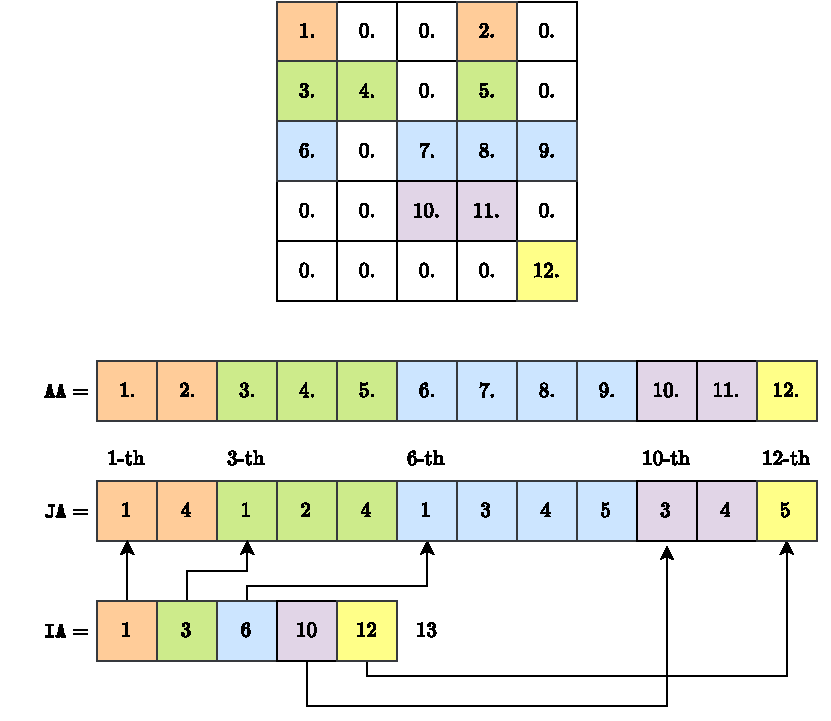
\includegraphics[width=\textwidth]{img/crs.pdf}
		\caption{View an illustration of the CRS technique using colors to improve readability.}
	\end{figure}
	\begin{figure}[!htp]
		\centering
		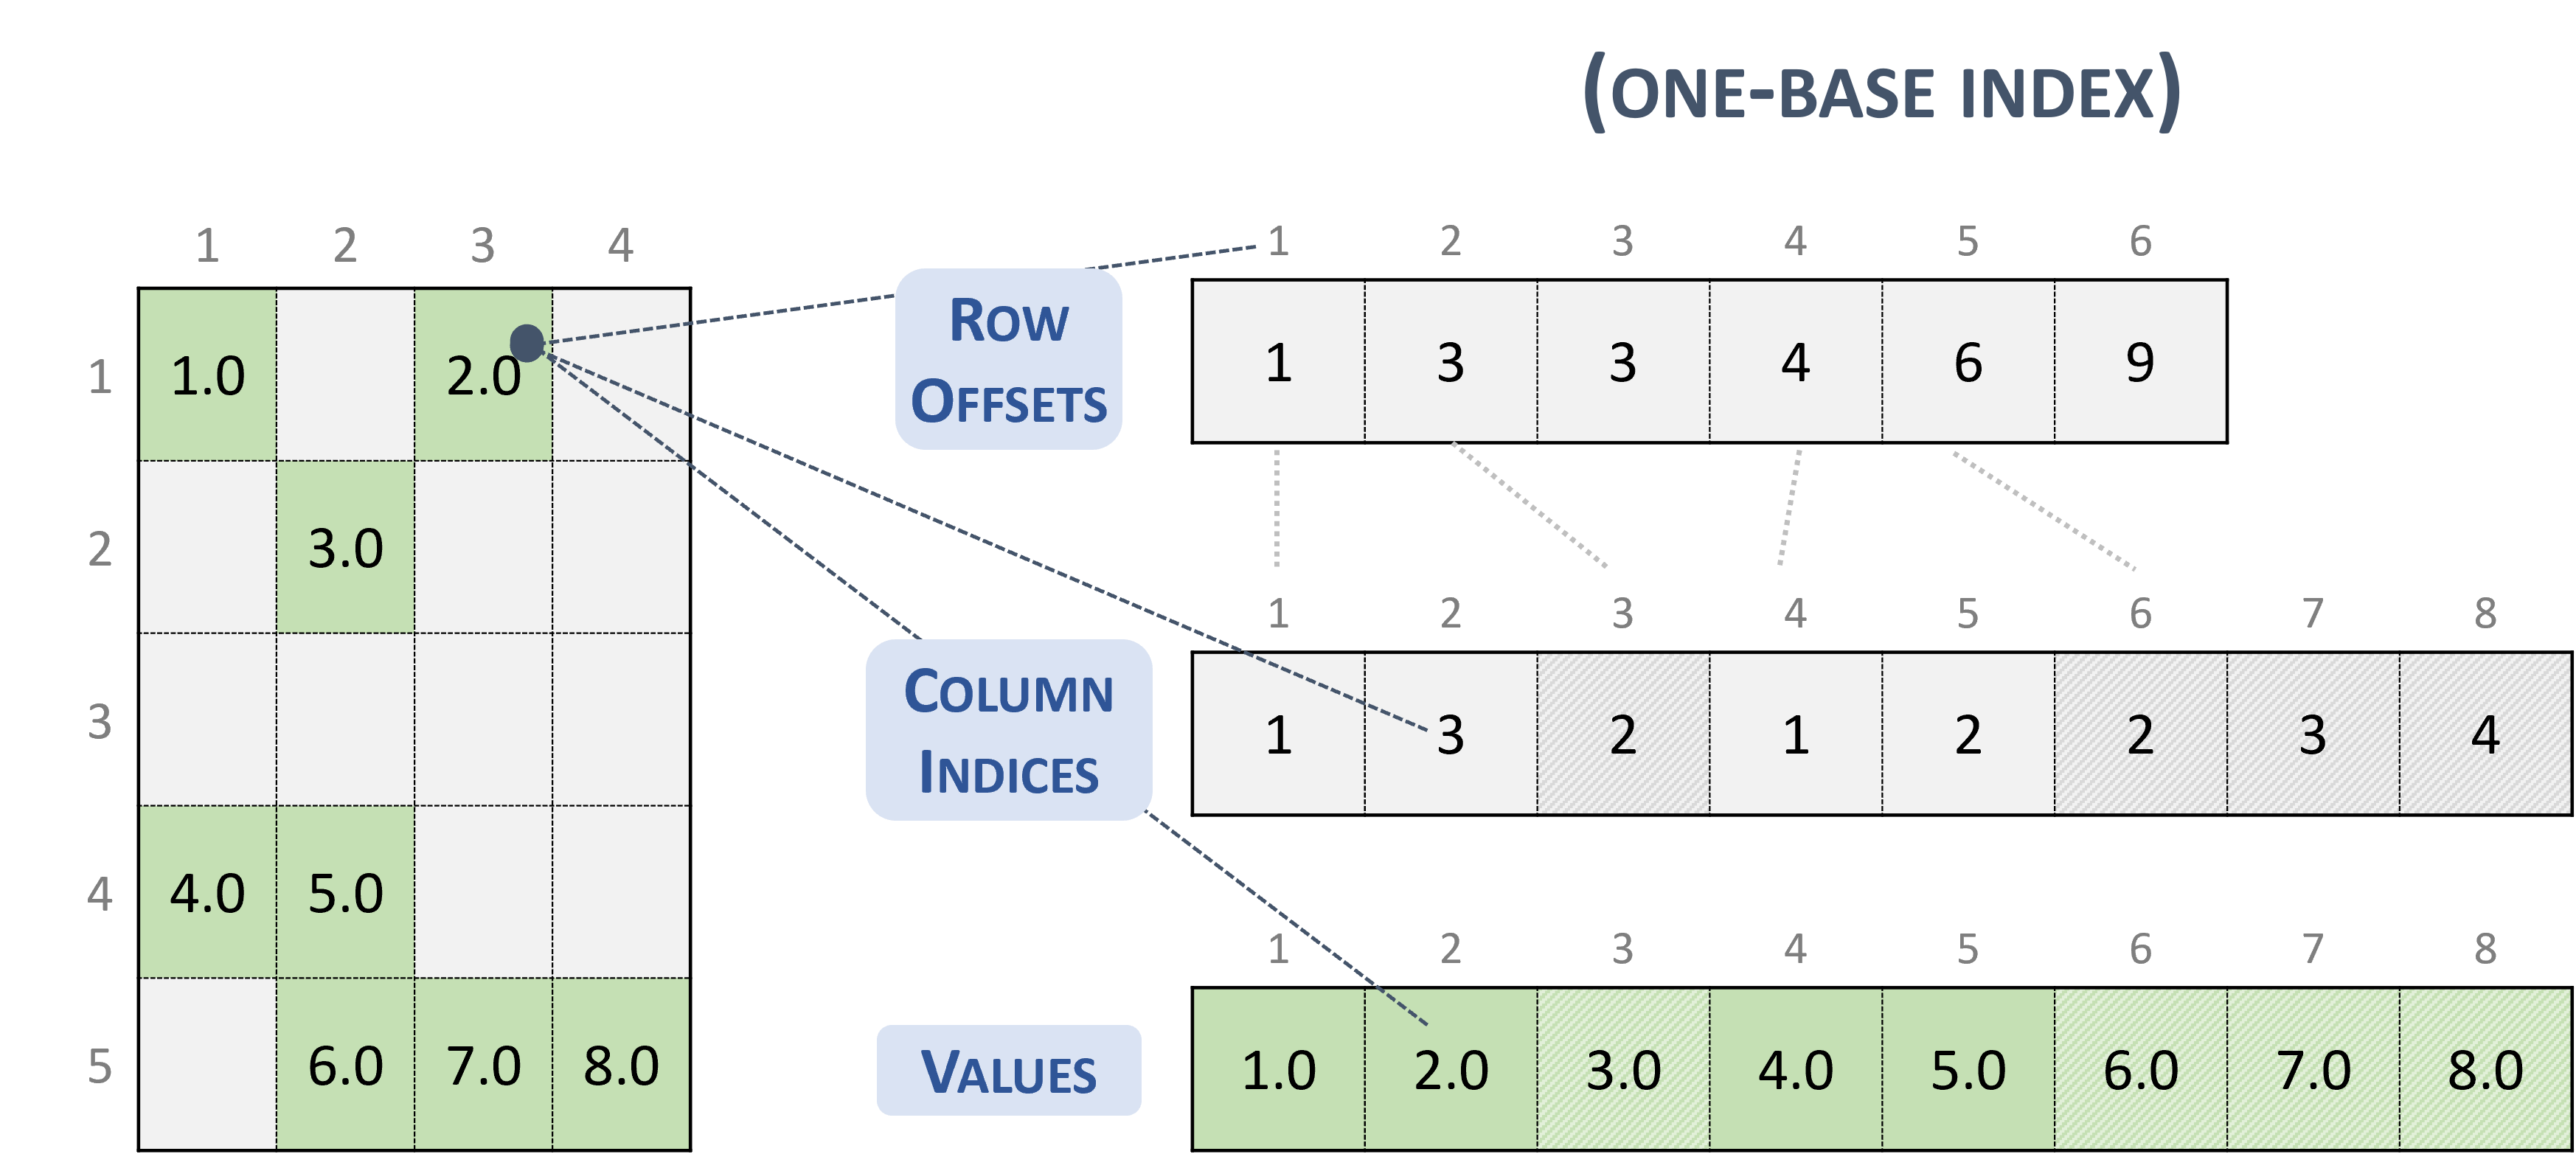
\includegraphics[width=.9\textwidth]{img/csr_one_base.png}
		\caption{Graphical representation of the coordinate compressed sparse row (CSR) technique. From the figure we can see the representation of the \texttt{AA} array, called \emph{values}, the \texttt{IA}, called \emph{row offset}, and finally the \texttt{JA}, called \emph{column indices}.
		It's interesting to see how the empty line case is handled. It copies the previous value of the array.
		The figures are taken from the \href{https://docs.nvidia.com/nvpl/_static/sparse/storage_format/sparse_matrix.html}{NVIDIA Performance Libraries Sparse}, which is part of the \href{https://developer.nvidia.com/nvpl}{NVIDIA Performance Libraries}.}
	\end{figure}
\end{itemize}

    %%%%%%%%%%%%%%%%%%%%%%%%%%
    % Bibliography and index %
    %%%%%%%%%%%%%%%%%%%%%%%%%%
    \pagestyle{fancy}
\fancyhead{} % clear all header fields
\fancyhead[R]{\nouppercase{\leftmark}}

\bibliography{bibtex}{}
\bibliographystyle{plain}

\newpage

\printindex
\end{document}